% cox and mullender, semaphores.
% 
% process has one thread with two stacks
%  
% pike et al, sleep and wakeup
\chapter{Scheduling}
\label{CH:SCHED}

Any operating system is likely to run with more processes than the
computer has CPUs, so a plan is needed to time-share the
CPUs among the processes. Ideally the sharing would be transparent to user
processes.  A common approach is to provide each process
with the illusion that it has its own virtual CPU by
\indextext{multiplexing}
the processes onto the hardware CPUs.
This chapter explains how xv6 achieves this multiplexing.
%% 
\section{Multiplexing}
%% 

Xv6 multiplexes by switching each CPU from one process to
another in two situations. First, xv6's
\lstinline{sleep}
and
\lstinline{wakeup}
mechanism switches when a process waits
for device or pipe I/O to complete, or waits for a child
to exit, or waits in the
\lstinline{sleep}
system call.
Second, xv6 periodically forces a switch to cope with
processes that compute for long periods without sleeping.
This multiplexing creates the illusion that
each process has its own CPU, much as xv6 uses the memory allocator and hardware
page tables to create the illusion that each process has its own memory.

Implementing multiplexing poses a few challenges. First, how to switch from one
process to another? 
Although the idea of context switching
is simple, the implementation is some of the most opaque code
in xv6. Second, how to force
switches in a way that is transparent to user processes?  Xv6 uses the
standard technique in which a hardware timer's interrupts drive context switches.
Third, all of the CPUs switch among the same shared set of processes, and a
locking plan is necessary to avoid races. Fourth, a process's
memory and other resources must be freed when the process exits,
but it cannot do all of this itself
because (for example) it can't free its own kernel stack while still using it.
Fifth, each core of a multi-core machine must remember which
process it is executing so that system calls affect the correct
process's kernel state.
Finally,  \lstinline{sleep} and \lstinline{wakeup} allow a process to give up
the CPU and wait to be woken up by another process or interrupt.
Care is needed to avoid races that result in
the loss of wakeup notifications.
Xv6 tries to solve these problems as
simply as possible, but nevertheless the resulting code is
tricky.

%% 
\section{Code: Context switching}
%% 

\begin{figure}[t]
\center
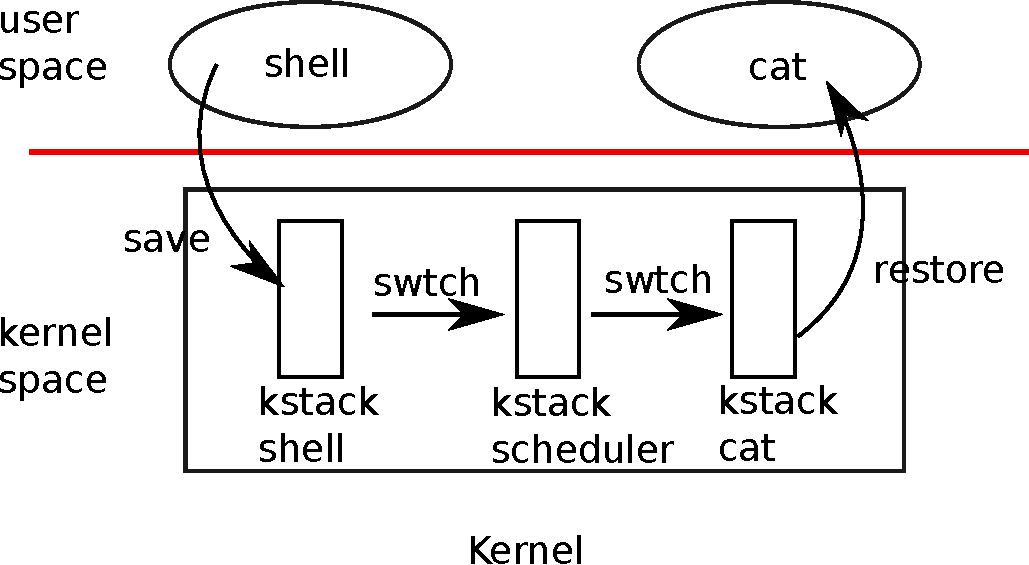
\includegraphics[scale=0.5]{fig/switch.pdf}
\caption{Switching from one user process to another.  In this example, xv6 runs with one CPU (and thus one scheduler thread).}
\label{fig:switch}
\end{figure}

Figure~\ref{fig:switch} 
outlines the steps involved in switching from one
user process to another:
a user-kernel transition (system
call or interrupt) to the old process's kernel thread,
a context switch to the current CPU's scheduler thread, a context
switch to a new process's kernel thread, and a trap return
to the user-level process.
The xv6 scheduler has a dedicated thread (saved registers and stack)
per CPU because
it is not safe for the scheduler execute on
the old process's kernel stack: some other core might
wake the process up and run it, and it would be a disaster
to use the same stack on two different cores.
%
% I think it may never be safe. if the old process is a ZOMBIE, the
% parent may mark it UNUSED and another core may allocate it in
% fork(). if the old process is SLEEPING or RUNNABLE, another core may
% wake it up and run it.
%
% what has changed is that, if we deleted wait(), it would 
% be safe for an exit()ing process to set its state to UNUSED
% directly (no ZOMBIE, no need for parent cleanup).
%
In this section we'll examine the mechanics of switching
between a kernel thread and a scheduler thread.

Switching from one thread to another involves saving the old thread's
CPU registers, and restoring the previously-saved registers of the
new thread; the fact that
the stack pointer and program counter
are saved and restored means that the CPU will switch stacks and
switch what code it is executing.

The function
\indexcode{swtch}
performs the saves and restores for a kernel thread switch.
\lstinline{swtch}
doesn't directly know about threads; it just saves and
restores sets of 32 RISC-V registers, called 
\indextext{contexts}.
When it is time for a process to give up the CPU,
the process's kernel thread calls
\lstinline{swtch}
to save its own context and return to the scheduler context.
Each context is contained in a
\lstinline{struct}
\lstinline{context}
\lineref{kernel/proc.h:/^struct.context/},
itself contained in a process's
\lstinline{struct proc}
or a CPU's
\lstinline{struct cpu}.
\lstinline{Swtch}
takes two arguments:
\indexcode{struct context}
\lstinline{*old}
and
\lstinline{struct}
\lstinline{context}
\lstinline{*new}.
It saves the current registers in
\lstinline{old},
loads registers from 
\lstinline{new},
and returns.

Let's follow a process through
\lstinline{swtch} 
into the scheduler.
We saw in Chapter~\ref{CH:TRAP}
that one possibility at the end of an interrupt is that 
\indexcode{usertrap}
calls 
\indexcode{yield}.
\lstinline{Yield}
in turn calls
\indexcode{sched},
which calls
\indexcode{swtch}
to save the current context in
\lstinline{p->context}
and switch to the scheduler context previously saved in 
\indexcode{cpu->scheduler}
\lineref{kernel/proc.c:/swtch..p/}.

\lstinline{Swtch}
\lineref{kernel/swtch.S:/swtch/}
saves only callee-saved registers;
the C compiler generates code in the caller to save
caller-saved registers on the stack.
\lstinline{Swtch} knows the offset of each
register's field in 
\lstinline{struct context}.
It does not save the program counter.
Instead,
\lstinline{swtch}
saves the
\lstinline{ra} register,
which holds the return address from which
\lstinline{swtch}
was called.
Now
\lstinline{swtch}
restores registers from the new context,
which holds register values saved by a previous
\lstinline{swtch}.
When 
\lstinline{swtch}
returns, it returns to the instructions pointed to
by the restored
\lstinline{ra}
register, that is,
the instruction from which the new thread previously
called \lstinline{swtch}.
In addition, it returns on the new thread's stack,
since that's where the restored \lstinline{sp} points.

In our example, 
\indexcode{sched}
called
\indexcode{swtch}
to switch to
\indexcode{cpu->scheduler},
the per-CPU scheduler context.
That context was saved at the point in the past when
\lstinline{scheduler}
called
\lstinline{swtch}
\lineref{kernel/proc.c:/swtch.&c/}
to switch to the process that's now giving up the CPU.
When the
\indexcode{swtch}
we have been tracing returns,
it returns not to
\lstinline{sched}
but to 
\indexcode{scheduler},
with the stack pointer in the current CPU's
scheduler stack.
%% 
\section{Code: Scheduling}
%% 

The last section looked at the low-level details of
\indexcode{swtch};
now let's take 
\lstinline{swtch}
as a given and examine 
switching from one process's kernel thread
through the scheduler to another process.
The scheduler exists in the form of a special thread per CPU, each running the
\lstinline{scheduler}
function.
This function is in charge of choosing which process to run next.
A process
that wants to give up the CPU must
acquire its own process lock
\indexcode{p->lock},
release any other locks it is holding,
update its own state
(\lstinline{p->state}),
and then call
\indexcode{sched}.
You can see this sequence in
\lstinline{yield}
\lineref{kernel/proc.c:/^yield/},
\texttt{sleep}
and
\texttt{exit}.
\lstinline{Sched}
double-checks some of those requirements
\linerefs{kernel/proc.c:/if..holding/,/running/}
and then checks an implication:
since a lock is held, interrupts should be disabled.
Finally,
\indexcode{sched}
calls
\indexcode{swtch}
to save the current context in 
\lstinline{p->context}
and switch to the scheduler context in
\indexcode{cpu->scheduler}.
\lstinline{Swtch}
returns on the scheduler's stack
as though
\indexcode{scheduler}'s
\lstinline{swtch}
had returned
\lineref{kernel/proc.c:/swtch.*schedul.*contex/}.
The scheduler continues its
\lstinline{for}
loop, finds a process to run, 
switches to it, and the cycle repeats.

We just saw that xv6 holds
\indexcode{p->lock}
across calls to
\lstinline{swtch}:
the caller of
\indexcode{swtch}
must already hold the lock, and control of the lock passes to the
switched-to code.  This convention is unusual with locks; usually
the thread that acquires a lock is also responsible for
releasing the lock, which makes it easier to reason about correctness.
For context switching it is necessary to break this convention because
\indexcode{p->lock}
protects invariants on the process's
\lstinline{state}
and
\lstinline{context}
fields that are not true while executing in
\lstinline{swtch}.
One example of a problem that could arise if
\lstinline{p->lock}
were not held during
\indexcode{swtch}:
a different CPU might decide
to run the process after 
\indexcode{yield}
had set its state to
\lstinline{RUNNABLE},
but before 
\lstinline{swtch}
caused it to stop using its own kernel stack.
The result would be two CPUs running on the same stack,
which cannot be right.

The only place a kernel thread gives up its CPU is in
\lstinline{sched},
and it always switches to the same location in \lstinline{scheduler}, which
(almost) always switches to some kernel thread that previously called
\lstinline{sched}. 
Thus, if one were to print out the line numbers where xv6 switches
threads, one would observe the following simple pattern:
\lineref{kernel/proc.c:/swtch..c/},
\lineref{kernel/proc.c:/swtch..p/},
\lineref{kernel/proc.c:/swtch..c/},
\lineref{kernel/proc.c:/swtch..p/},
and so on.
Procedures that intentionally transfer control to each other via thread
switch are sometimes referred to as
\indextext{coroutines}; 
in this example,
\indexcode{sched}
and
\indexcode{scheduler}
are co-routines of each other.

There is one case when the scheduler's call to
\indexcode{swtch}
does not end up in
\indexcode{sched}.
\lstinline{allocproc} sets the context \lstinline{ra}
register of a new process to
\indexcode{forkret}
\lineref{kernel/proc.c:/^forkret/},
so that its first \lstinline{swtch} ``returns'' 
to the start of that function.
\lstinline{Forkret}
exists to release the 
\indexcode{p->lock};
otherwise, since the new process needs to
return to user space as if returning from \lstinline{fork},
it could instead start at
\lstinline{usertrapret}.

\lstinline{Scheduler}
\lineref{kernel/proc.c:/^scheduler/} 
runs a loop:
find a process to run, run it until it yields, repeat.
The scheduler
loops over the process table
looking for a runnable process, one that has
\lstinline{p->state} 
\lstinline{==}
\lstinline{RUNNABLE}.
Once it finds a process, it sets the per-CPU current process
variable
\lstinline{c->proc},
marks the process as
\lstinline{RUNNING},
and then calls
\indexcode{swtch}
to start running it
\linerefs{kernel/proc.c:/Switch.to/,/swtch/}.

One way to think about the structure of the scheduling code is
that it enforces a set of invariants about each process,
and holds
\indexcode{p->lock}
whenever those invariants are not true.
One invariant is that if a process is
\lstinline{RUNNING},
a timer interrupt's
\indexcode{yield}
must be able to safely switch away from the process;
this means that the CPU registers must hold the process's register values
(i.e. 
\lstinline{swtch}
hasn't moved them to a
\lstinline{context}),
and
\lstinline{c->proc}
must refer to the process.
Another invariant is that if a process is
\indexcode{RUNNABLE},
it must be safe for
an idle CPU's
\indexcode{scheduler}
to run it;
this means that 
\indexcode{p->context}
must hold the process's registers (i.e., they are
not actually in the real registers),
that no CPU is executing on the process's kernel stack,
and that no CPU's
\lstinline{c->proc}
refers to the process.
Observe that these properties are often not true while
\lstinline{p->lock} is held.

Maintaining the above invariants is the reason why xv6 often acquires 
\indexcode{p->lock}
in one thread and releases it in another,
for example acquiring in
\lstinline{yield}
and releasing in
\lstinline{scheduler}.
Once \lstinline{yield} has started to modify a running process's state
to make it
\lstinline{RUNNABLE},
the lock must remain held until the invariants are restored:
the earliest correct release point is after
\lstinline{scheduler}
(running on its own stack)
clears
\lstinline{c->proc}.
Similarly, once 
\lstinline{scheduler}
starts to convert a \lstinline{RUNNABLE} process to
\lstinline{RUNNING},
the lock cannot be released until the kernel thread
is completely running (after the
\lstinline{swtch},
for example in
\lstinline{yield}).

\indexcode{p->lock}
protects other things as well:
the interplay between
\indexcode{exit}
and
\indexcode{wait},
the machinery to avoid lost wakeups (see Section~\ref{sec:sleep}),
and avoidance of races between a process exiting and other processes
reading or writing its state (e.g., the \lstinline{exit}
system call looking at \lstinline{p->pid} and
setting \lstinline{p->killed}
\lineref{kernel/proc.c:/^kill/}).
It's possible that with some design effort the
different functions of
\lstinline{p->lock}
could be split up, for clarity and perhaps
for performance.
%% 
\section{Code: mycpu and myproc}
%% 

Xv6 often needs a pointer to the current process's \lstinline{proc}
structure. On a uniprocessor one could have a global variable pointing
to the current \lstinline{proc}. This doesn't work on a multi-core
machine, since each core executes a different process. The way to
solve this problem is to exploit the fact that each core has its own
set of registers; we can use one of those registers to help find
per-core information.

Xv6 maintains a
\indexcode{struct cpu}
for each CPU
\lineref{kernel/proc.h:/^struct.cpu/},
which records
the process currently running
on that CPU (if any),
saved registers for the CPU's scheduler thread,
and the count of nested spinlocks needed to manage
interrupt disabling.
The function
\indexcode{mycpu}
\lineref{kernel/proc.c:/^mycpu/}
returns a pointer to the current CPU's
\lstinline{struct cpu}.
RISC-V numbers its CPUs, giving each
a \indextext{hartid}.
Xv6 ensures that each CPU's hartid is stored in that CPU's \lstinline{tp} register
while in the kernel.
This allows
\lstinline{mycpu} to use \lstinline{tp} to index an array
of \lstinline{cpu} structures to find the right one.

Ensuring that a CPU's \lstinline{tp} always holds the CPU's
hartid is a little involved. \lstinline{mstart} sets the \lstinline{tp}
register early in the CPU's boot sequence, while still in machine mode
\lineref{kernel/start.c:/w_tp/}.
\lstinline{usertrapret} saves \lstinline{tp} in the trampoline
page, because the user process might modify \lstinline{tp}.
Finally, \lstinline{uservec} restores that saved \lstinline{tp}
when entering the kernel from user space
\lineref{kernel/trampoline.S:/make tp hold/}.
The compiler guarantees never to use the \lstinline{tp}
register.
It would be more convenient if xv6 could ask the RISC-V
hardware for the current hartid whenever needed,
but RISC-V allows that only in
machine mode, not in supervisor mode.

The return values of
\lstinline{cpuid}
and
\lstinline{mycpu}
are fragile: if the timer were to interrupt and cause
the thread to yield and then move to a different CPU,
a previously returned value would no longer be correct.
To avoid this problem, xv6 requires that callers 
disable interrupts, and only enable
them after they finish using the returned
\lstinline{struct cpu}.

The function
\indexcode{myproc}
\lineref{kernel/proc.c:/^myproc/}
returns the
\lstinline{struct proc}
pointer
for the process that is running on the current CPU.
\lstinline{myproc}
disables interrupts, invokes
\lstinline{mycpu},
fetches the current process pointer
(\lstinline{c->proc})
out of the
\lstinline{struct cpu},
and then enables interrupts.
The return value of
\lstinline{myproc}
is safe to use even if interrupts are enabled:
if a timer interrupt moves the calling process to a
different CPU, its
\lstinline{struct proc}
pointer will stay the same.
%% 
\section{Sleep and wakeup}
\label{sec:sleep}
%% 

Scheduling and locks help conceal the actions of one thread
from another,
but we also need abstractions that help
threads intentionally interact.
For example, the reader of a pipe in xv6 may need to wait
for a writing process to produce data;
a parent's call to \lstinline{wait} may need to
wait for a child to exit; and
a process reading the disk needs to wait
for the disk hardware to finish the read.
The xv6 kernel uses a mechanism called sleep and wakeup
in these situations (and many others).
Sleep allows a kernel thread to
wait for a specific event; another thread can call wakeup 
to indicate that threads waiting for an event should resume.
Sleep and wakeup are often called 
\indextext{sequence coordination}
or 
\indextext{conditional synchronization}
mechanisms.

Sleep and wakeup provide a relatively low-level synchronization
interface. To motivate the way they work in xv6,
we'll use them to build a higher-level
synchronization mechanism called a \indextext{semaphore}~\cite{dijkstra65} that
coordinates producers and consumers
(xv6 does not use semaphores).
A semaphore maintains a count and provides two operations.
The ``V'' operation (for the producer) increments the count.
The ``P'' operation (for the consumer) waits until the count is non-zero,
and then decrements it and returns.
If there were only one producer thread and one consumer thread,
and they executed on different CPUs,
and the compiler didn't optimize too aggressively,
this implementation would be correct:
\begin{lstlisting}[numbers=left,firstnumber=100]
  struct semaphore {
    struct spinlock lock;
    int count;
  };

  void
  V(struct semaphore *s)
  {
     acquire(&s->lock);
     s->count += 1;
     release(&s->lock);
  }

  void
  P(struct semaphore *s)
  {
     while(s->count == 0)
       ;
     acquire(&s->lock);
     s->count -= 1;
     release(&s->lock);
  }
\end{lstlisting}

The implementation above 
is expensive.  If the producer acts
rarely, the consumer will spend most
of its time spinning in the 
\lstinline{while}
loop hoping for a non-zero count.
The consumer's CPU could probably find more productive work than 
\indextext{busy waiting}
by repeatedly 
\indextext{polling}
\lstinline{s->count}.
Avoiding busy waiting requires
a way for the consumer to yield the CPU
and resume only after
\lstinline{V}
increments the count.

Here's a step in that direction, though as we
will see it is not enough.
Let's imagine a pair of calls, 
\indexcode{sleep}
and
\indexcode{wakeup},
that work as follows.
\lstinline{Sleep(chan)}
sleeps on the arbitrary value
\indexcode{chan},
called the 
\indextext{wait channel}.
\lstinline{Sleep}
puts the calling process to sleep, releasing the CPU
for other work.
\lstinline{Wakeup(chan)}
wakes all processes sleeping on
\lstinline{chan}
(if any), causing their
\lstinline{sleep}
calls to return.
If no processes are waiting on
\lstinline{chan},
\lstinline{wakeup}
does nothing.
We can change the semaphore implementation to use
\lstinline{sleep}
and
\lstinline{wakeup} (changes highlighted in yellow):
\begin{lstlisting}[numbers=left,firstnumber=200]
  void
  V(struct semaphore *s)
  {
     acquire(&s->lock);
     s->count += 1;
     (*@\hl{wakeup(s);}@*)
     release(&s->lock);
  }
  
  void
  P(struct semaphore *s)
  {
    while(s->count == 0)    (*@\label{line:test}@*)
      (*@\hl{sleep(s);}@*)  (*@\label{line:sleep}@*)
    acquire(&s->lock);
    s->count -= 1;
    release(&s->lock);
  }
\end{lstlisting}

% \begin{figure}[t]
% \center
% 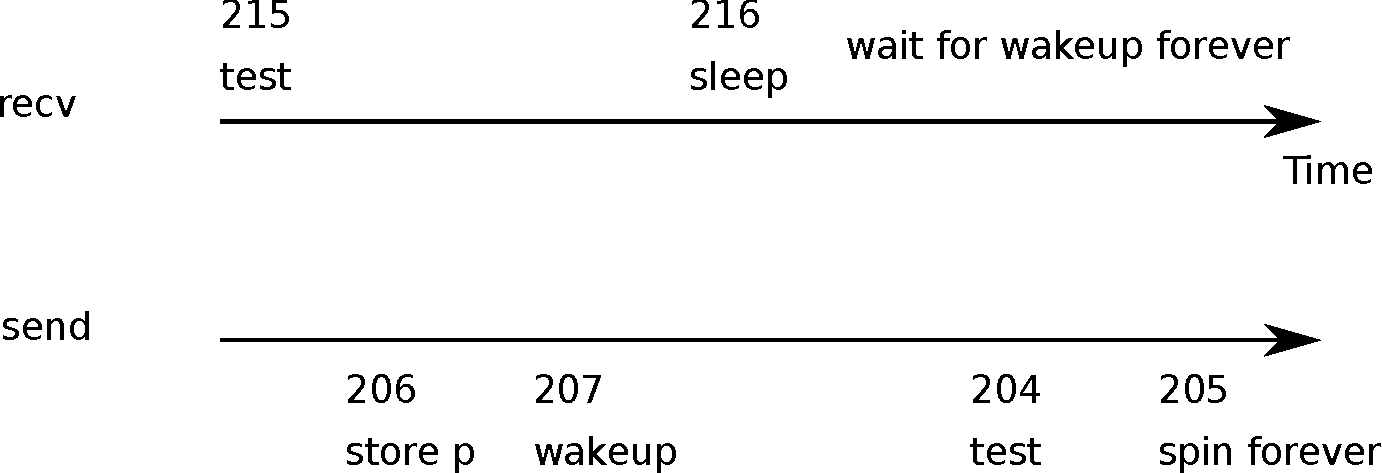
\includegraphics[scale=0.5]{fig/deadlock.pdf}
% \caption{Example lost wakeup problem}
% \label{fig:deadlock}
% \end{figure}

\lstinline{P}
now gives up the CPU instead of spinning, which is nice.
However, it turns out not to be straightforward to design
\lstinline{sleep}
and 
\lstinline{wakeup}
with this interface without suffering
from what is known as the \indextext{lost wake-up} problem.
% (see 
% Figure~\ref{fig:deadlock}).
Suppose that
\lstinline{P}
finds that
\lstinline{s->count}
\lstinline{==}
\lstinline{0} 
on line~\ref{line:test}.
While
\lstinline{P}
is between lines~\ref{line:test} and~\ref{line:sleep},
\lstinline{V}
runs on another CPU:
it changes
\lstinline{s->count}
to be nonzero and calls
\lstinline{wakeup},
which finds no processes sleeping and thus does nothing.
Now
\lstinline{P}
continues executing at line~\ref{line:sleep}:
it calls
\lstinline{sleep}
and goes to sleep.
This causes a problem:
\lstinline{P}
is asleep waiting for a \lstinline{V} call
that has already happened.
Unless we get lucky and the producer calls
\lstinline{V} again, the consumer will wait
forever even
though the count is non-zero.

The root of this problem is that the
invariant that
\lstinline{P}
only sleeps when
\lstinline{s->count}
\lstinline{==}
\lstinline{0}
is violated by 
\lstinline{V}
running at just the wrong moment.
An incorrect way to protect the invariant would be to 
move the lock acquisition (highlighted in yellow below) in
\lstinline{P}
so that its check of the count and its call to \lstinline{sleep}
are atomic:
\begin{lstlisting}[numbers=left,firstnumber=300]
  void
  V(struct semaphore *s)
  {
    acquire(&s->lock);
    s->count += 1;
    wakeup(s);
    release(&s->lock);
  }
  
  void
  P(struct semaphore *s)
  {
    (*@\hl{acquire(\&s->lock);}@*)
    while(s->count == 0)    (*@\label{line:test1}@*)
      sleep(s);             (*@\label{line:sleep1}@*)
    s->count -= 1;
    release(&s->lock);
  }
\end{lstlisting}
One might hope that this version of
\lstinline{P}
would avoid the lost wakeup because the lock prevents
\lstinline{V}
from executing between lines~\ref{line:test1} and~\ref{line:sleep1}.
It does that, but it also deadlocks:
\lstinline{P}
holds the lock while it sleeps,
so \lstinline{V} will block forever waiting for the lock.

We'll fix the preceding scheme by changing
\lstinline{sleep}'s
interface:
the caller must pass the \indextext{condition lock} to
\lstinline{sleep}
so it can release the lock after
the calling process is marked as asleep and waiting on the
sleep channel.
The lock will force a concurrent
\lstinline{V}
to wait until \lstinline{P} has finished putting itself to sleep,
so that the
\lstinline{wakeup}
will find the sleeping consumer and wake it up.
Once the consumer is awake again
\indexcode{sleep}
reacquires the lock before returning.
Our new correct sleep/wakeup scheme is usable as follows (change
highlighted in yellow):
\begin{lstlisting}[numbers=left,firstnumber=400]
  void
  V(struct semaphore *s)
  {
    acquire(&s->lock);
    s->count += 1;
    wakeup(s);
    release(&s->lock);
  }

  void
  P(struct semaphore *s)
  {
    acquire(&s->lock);
    while(s->count == 0)
       (*@\hl{sleep(s, \&s->lock);}@*)
    s->count -= 1;
    release(&s->lock);
  }
\end{lstlisting}

The fact that
\lstinline{P}
holds
\lstinline{s->lock}
prevents 
\lstinline{V}
from trying to wake it up between 
\lstinline{P}'s
check of
\lstinline{c->count}
and its call to
\lstinline{sleep}.
Note, however, that we need
\lstinline{sleep}
to atomically release
\lstinline{s->lock}
and put the consuming process to sleep,
in order to avoid lost wakeups.

%% 
\section{Code: Sleep and wakeup}
%% 

Xv6's
\indexcode{sleep}
\lineref{kernel/proc.c:/^sleep/}
and
\indexcode{wakeup}
\lineref{kernel/proc.c:/^wakeup/}
provide the interface shown in the last example above,
and their implementation (plus rules for how to use them)
ensures that there are no lost wakeups.
The basic idea is to have
\lstinline{sleep}
mark the current process as
\indexcode{SLEEPING}
and then call
\indexcode{sched}
to release the CPU;
\lstinline{wakeup}
looks for a process sleeping on the given wait channel
and marks it as 
\indexcode{RUNNABLE}.
Callers of
\lstinline{sleep}
and
\lstinline{wakeup}
can use any mutually convenient number as the channel.
Xv6 often uses the address
of a kernel data structure involved in the waiting.

\lstinline{Sleep}
acquires 
\indexcode{p->lock}
\lineref{kernel/proc.c:/DOC: sleeplock1/}.
Now the process going to sleep holds both
\lstinline{p->lock}
and
\lstinline{lk}.
Holding
\lstinline{lk}
was necessary in the caller (in the example,
\lstinline{P}):
it
ensured that no other process (in the example,
one running
\lstinline{V})
could start a call to
\lstinline{wakeup(chan)}.
Now that
\lstinline{sleep}
holds
\lstinline{p->lock},
it is safe to release
\lstinline{lk}:
some other process may start a call to
\lstinline{wakeup(chan)},
but
\indexcode{wakeup}
will wait to acquire
\indexcode{p->lock},
and thus will wait until
\lstinline{sleep}
has finished putting the process to sleep,
keeping the
\lstinline{wakeup}
from missing the
\lstinline{sleep}.

There is a minor complication: if 
\lstinline{lk}
is in fact
\lstinline{p->lock},
then
\lstinline{sleep}
would deadlock with itself if it tried to acquire 
\lstinline{p->lock}.
But if the process calling
\lstinline{sleep}
already holds \lstinline{p->lock}, it
doesn't need to do anything more in order
to avoiding missing a concurrent \lstinline{wakeup}.
This case arises when
\lstinline{wait}
\lineref{kernel/proc.c:/^wakeup\(/}
calls
\lstinline{sleep}
with 
\lstinline{p->lock}.

Now that
\lstinline{sleep}
holds
\lstinline{p->lock}
and no others,
it can put the process to sleep by recording
the sleep channel,
changing the process state to \texttt{SLEEPING},
and calling
\lstinline{sched}
\linerefs{kernel/proc.c:/chan.=.chan/,/sched/}.
In a moment it will be clear why it's critical that
\lstinline{p->lock} is not released (by \lstinline{scheduler}) until after
the process is marked \texttt{SLEEPING}.

At some point, a process will acquire the condition lock,
set the condition that the sleeper is waiting for,
and call \lstinline{wakeup(chan)}.
It's important that \lstinline{wakeup} is called
while holding the condition lock\footnote{%
%
Strictly speaking it is sufficient if
\lstinline{wakeup}
merely follows the
\lstinline{acquire}
(that is, one could call
\lstinline{wakeup}
after the
\lstinline{release}).%
%
}.
\lstinline{Wakeup}
loops over the process table
\lineref{kernel/proc.c:/^wakeup\(/}.
It acquires the
\lstinline{p->lock}
of each process it inspects,
both because it may manipulate that process's state
and because
\lstinline{p->lock}
ensures that
\lstinline{sleep}
and
\lstinline{wakeup}
do not miss each other.
When \lstinline{wakeup} finds a process in state
\indexcode{SLEEPING}
with a matching
\indexcode{chan},
it changes that process's state to
\indexcode{RUNNABLE}.
The next time the scheduler runs, it will
see that the process is ready to be run.

Why do the locking rules for 
\lstinline{sleep}
and
\lstinline{wakeup}
ensure a sleeping process won't miss a wakeup?
The sleeping process holds either
the condition lock or its own
\lstinline{p->lock} 
or both from a point before it checks the condition
to a point after it is marked \texttt{SLEEPING}.
The process calling \texttt{wakeup} holds \textit{both}
of those locks in \texttt{wakeup}'s loop.
Thus the waker either makes the condition true before
the consuming thread checks the condition;
or the waker's \lstinline{wakeup} examines the sleeping
thread strictly after it has been marked \texttt{SLEEPING}.
Then 
\lstinline{wakeup}
will see the sleeping process and wake it up
(unless something else wakes it up first).

It is sometimes the case that multiple processes are sleeping
on the same channel; for example, more than one process
reading from a pipe.
A single call to 
\lstinline{wakeup}
will wake them all up.
One of them will run first and acquire the lock that
\lstinline{sleep}
was called with, and (in the case of pipes) read whatever
data is waiting in the pipe.
The other processes will find that, despite being woken up,
there is no data to be read.
From their point of view the wakeup was ``spurious,'' and
they must sleep again.
For this reason \lstinline{sleep} is always called inside a loop that
checks the condition.

No harm is done if two uses of sleep/wakeup accidentally
choose the same channel: they will see spurious wakeups,
but looping as described above will tolerate this problem.
Much of the charm of sleep/wakeup is that it is both
lightweight (no need to create special data
structures to act as sleep channels) and provides a layer
of indirection (callers need not know which specific process
they are interacting with).
%% 
\section{Code: Pipes}
%% 
A more complex example that uses \lstinline{sleep}
and \lstinline{wakeup} to synchronize producers and
consumers is xv6's implementation of pipes.
We saw the interface for pipes in Chapter~\ref{CH:UNIX}:
bytes written to one end of a pipe are copied
to an in-kernel buffer and then can be read from
the other end of the pipe.
Future chapters will examine the file descriptor support
surrounding pipes, but let's look now at the
implementations of 
\indexcode{pipewrite}
and
\indexcode{piperead}.

Each pipe
is represented by a 
\indexcode{struct pipe},
which contains
a 
\lstinline{lock}
and a 
\lstinline{data}
buffer.
The fields
\lstinline{nread}
and
\lstinline{nwrite}
count the total number of bytes read from
and written to the buffer.
The buffer wraps around:
the next byte written after
\lstinline{buf[PIPESIZE-1]}
is 
\lstinline{buf[0]}.
The counts do not wrap.
This convention lets the implementation
distinguish a full buffer 
(\lstinline{nwrite}
\lstinline{==}
\lstinline{nread+PIPESIZE})
from an empty buffer
(\lstinline{nwrite}
\lstinline{==}
\lstinline{nread}),
but it means that indexing into the buffer
must use
\lstinline{buf[nread}
\lstinline{%}
\lstinline{PIPESIZE]}
instead of just
\lstinline{buf[nread]} 
(and similarly for
\lstinline{nwrite}).

Let's suppose that calls to
\lstinline{piperead}
and
\lstinline{pipewrite}
happen simultaneously on two different CPUs.
\lstinline{Pipewrite}
\lineref{kernel/pipe.c:/^pipewrite/}
begins by acquiring the pipe's lock, which
protects the counts, the data, and their
associated invariants.
\lstinline{Piperead}
\lineref{kernel/pipe.c:/^piperead/}
then tries to acquire the lock too, but cannot.
It spins in
\lstinline{acquire}
\lineref{kernel/spinlock.c:/^acquire/}
waiting for the lock.
While
\lstinline{piperead}
waits,
\lstinline{pipewrite}
loops over the bytes being written
(\lstinline{addr[0..n-1]}),
adding each to the pipe in turn
\lineref{kernel/pipe.c:/nwrite\+\+/}.
During this loop, it could happen that
the buffer fills
\lineref{kernel/pipe.c:/DOC: pipewrite-full/}.
In this case, 
\lstinline{pipewrite}
calls
\lstinline{wakeup}
to alert any sleeping readers to the fact
that there is data waiting in the buffer
and then sleeps on
\lstinline{&pi->nwrite}
to wait for a reader to take some bytes
out of the buffer.
\lstinline{Sleep}
releases 
\lstinline{pi->lock}
as part of putting
\lstinline{pipewrite}'s
process to sleep.

Now that
\lstinline{pi->lock}
is available,
\lstinline{piperead}
manages to acquire it and enters its critical section:
it finds that
\lstinline{pi->nread}
\lstinline{!=}
\lstinline{pi->nwrite}
\lineref{kernel/pipe.c:/DOC: pipe-empty/}
(\lstinline{pipewrite}
went to sleep because
\lstinline{pi->nwrite}
\lstinline{==}
\lstinline{pi->nread+PIPESIZE}
\lineref{kernel/pipe.c:/pipewrite-full/}),
so it falls through to the 
\lstinline{for}
loop, copies data out of the pipe
\lineref{kernel/pipe.c:/DOC: piperead-copy/},
and increments 
\lstinline{nread}
by the number of bytes copied.
That many bytes are now available for writing, so
\lstinline{piperead}
calls
\lstinline{wakeup}
\lineref{kernel/pipe.c:/DOC: piperead-wakeup/}
to wake any sleeping writers
before it returns.
\lstinline{Wakeup}
finds a process sleeping on
\lstinline{&pi->nwrite},
the process that was running
\lstinline{pipewrite}
but stopped when the buffer filled.
It marks that process as
\indexcode{RUNNABLE}.

The pipe code uses separate sleep channels for reader and writer
(\lstinline{pi->nread}
and
\lstinline{pi->nwrite});
this might make the system more efficient in the unlikely
event that there are lots of
readers and writers waiting for the same pipe.
The pipe code sleeps inside a loop checking the
sleep condition; if there are multiple readers
or writers, all but the first process to wake up
will see the condition is still false and sleep again.
%% 
\section{Code: Wait, exit, and kill}
%% 
\lstinline{Sleep}
and
\lstinline{wakeup}
can be used for many kinds of waiting.
An interesting example, introduced in Chapter~\ref{CH:UNIX},
is the interaction between a child's \indexcode{exit}
and its parent's \indexcode{wait}.
At the time of the child's death, the parent may already
be sleeping in {\tt wait}, or may be doing something else;
in the latter case, a subsequent call to {\tt wait} must
observe the child's death, perhaps long after it calls {\tt exit}.
The way that xv6 records the child's demise until {\tt wait}
observes it is for {\tt exit} to put the caller into the \indexcode{ZOMBIE}
state, where it stays until the parent's {\tt wait} notices it, changes
the child's state to {\tt UNUSED}, copies the child's exit status,
and returns the child's process ID to the parent.
If the parent exits before the child, the 
parent gives the child to the
\lstinline{init}
process, which perpetually calls {\tt wait};
thus
every child has a parent to clean up after it.
The main implementation challenge is
the possibility of races and deadlock between
parent and child
\lstinline{wait}
and
\lstinline{exit},
as well as
\lstinline{exit}
and
\lstinline{exit}.

\lstinline{Wait}
uses the calling process's
\lstinline{p->lock}
as the condition lock to avoid lost wakeups,
and it acquires that lock at the start
\lineref{kernel/proc.c:/^wait/}.
Then it scans the process table.
If it finds a child in \texttt{ZOMBIE} state,
it frees that child's resources and
its \lstinline{proc} structure, copies
the child's exit status to the address supplied to \lstinline{wait}
(if it is not 0),
and returns the child's process ID.
If 
\lstinline{wait}
finds children but none have exited,
it calls
\lstinline{sleep}
to wait for any of them to exit
\lineref{kernel/proc.c:/DOC: wait-sleep/},
then scans again.
Here,
the condition lock being released in 
\lstinline{sleep}
is the waiting process's \lstinline{p->lock},
the special case mentioned above.
Note that \lstinline{wait} often holds two locks;
that it acquires its own lock before trying to acquire
any child's lock;
and that thus all of xv6 must obey the same locking order
(parent, then child) in order to avoid deadlock.

\lstinline{Wait}
looks at every process's \lstinline{np->parent} to find
its children. It uses \lstinline{np->parent} without holding
\lstinline{np->lock}, which is a violation of the usual rule that
shared variables must be protected by locks. It is possible that
\lstinline{np} is an ancestor of the current process, in which case
acquiring \lstinline{np->lock} could cause a deadlock since that would
violate the locking order mentioned above. Examining \lstinline{np->parent}
without a lock seems safe in this case; a process's \lstinline{parent}
field is only changed by its parent, so if \lstinline{np->parent==p}
is true, the value can't change unless the current process changes it.

\lstinline{Exit}
\lineref{kernel/proc.c:/^exit/}
records the exit status, frees some resources,
gives any children to the \lstinline{init} process,
wakes up the parent in case it is in \lstinline{wait},
marks the caller as a zombie, and permanently
yields the CPU.
The final sequence is a little tricky.
The exiting process must hold its parent's lock while
it sets its state to \lstinline{ZOMBIE} and
wakes the parent up, since the parent's lock
is the condition lock
that guards against lost wakeups in \lstinline{wait}. The child must also
hold its own \lstinline{p->lock}, since otherwise the parent
might see it in state \lstinline{ZOMBIE} and free it while
it is still running.
The lock acquisition order is important to avoid deadlock: since \lstinline{wait}
acquires the parent's lock before the child's lock,
\lstinline{exit} must use the same order.

\lstinline{Exit} cannot call \lstinline{wakeup} to
wake a waiting parent, since \lstinline{wakeup}
aquires locks that would violate the parent-then-child locking order.
Instead,
\lstinline{exit} calls a specialized wakeup function,
\lstinline{wakeup1}, that does not acquire locks.
\lstinline{wakeup1} wakes up only the parent,
and only if it is sleeping in 
\lstinline{wait}
\lineref{kernel/proc.c:/^wakeup1/}.
It may look incorrect for the child to wake up the parent
before setting its state to \lstinline{ZOMBIE}, 
but that is safe:
although
\lstinline{wakeup1}
may cause the parent to run,
the loop in
\lstinline{wait}
cannot examine the child until the child's
\lstinline{p->lock}
is released by {\tt scheduler},
so
\lstinline{wait}
can't look at
the exiting process until well after
\lstinline{exit}
has set its state to
\lstinline{ZOMBIE}
\lineref{kernel/proc.c:/state.=.ZOMBIE/}.

While
\lstinline{exit} 
allows a process to terminate itself,
\lstinline{kill}
\lineref{kernel/proc.c:/^kill/} 
lets one process request that another terminate.
It would be too complex for
\lstinline{kill}
to directly destroy the victim process, since the victim
might be executing on another CPU, perhaps
in the middle of a sensitive sequence of updates to kernel data structures.
Thus
\lstinline{kill}
does very little: it just sets the victim's
\indexcode{p->killed}
and, if it is sleeping, wakes it up.
Eventually the victim will enter or leave the kernel,
at which point code in
\lstinline{usertrap}
will call
\lstinline{exit}
if
\lstinline{p->killed}
is set.
If the victim is running in user space, it will soon enter
the kernel by making a system call or because the timer (or
some other device) interrupts.

If the victim process is in
\lstinline{sleep},
\lstinline{kill}'s call to
\lstinline{wakeup}
will cause the victim to return from
\lstinline{sleep}.
This is potentially dangerous because 
the condition being waiting for may not be true.
However, xv6 calls to
\lstinline{sleep}
are always wrapped in a
\lstinline{while}
loop that re-tests the condition after
\lstinline{sleep}
returns.
Some calls to
\lstinline{sleep}
also test
\lstinline{p->killed}
in the loop, and abandon the current activity if it is set.
This is only done when such abandonment would be correct.
For example, the pipe read and write code
\lineref{kernel/pipe.c:/myproc..-\>killed/} 
returns if the killed flag is set; eventually the
code will return back to trap, which will again
check \lstinline{p->killed} and exit.

Some xv6 
\lstinline{sleep}
loops do not check
\lstinline{p->killed} 
because the code is in the middle of a multi-step
system call that should be atomic.
The virtio driver
\lineref{kernel/virtio\_disk.c:/sleep.b/} 
is an example: it does not check
\lstinline{p->killed}
because a disk operation may be one of a set of
writes that are all needed in order for the file system to
be left in a correct state.
A process that is killed while waiting for disk I/O won't
exit until it completes the current system call and
\lstinline{usertrap} sees the killed flag.
%% 
\section{Real world}
%% 

The xv6 scheduler implements a simple scheduling policy, which runs each process
in turn.  This policy is called
\indextext{round robin}.
Real operating systems implement more sophisticated policies that, for example,
allow processes to have priorities.  The idea is that a runnable high-priority process
will be preferred by the scheduler over a runnable low-priority process.   These
policies can become complex quickly because there are often competing goals: for
example, the operating might also want to guarantee fairness and
high throughput.  In addition, complex policies may lead to unintended
interactions such as
\indextext{priority inversion}
and 
\indextext{convoys}.
Priority inversion can happen when a low-priority and high-priority process
both use a particular lock, which when acquired by the low-priority process can prevent the
high-priority process from making progress.  A long convoy of waiting processes
can form when many
high-priority processes are waiting for a low-priority process that acquires a
shared lock; once a convoy has formed it can persist for long time.
To avoid these kinds of problems additional mechanisms are necessary in
sophisticated schedulers.

\lstinline{Sleep}
and
\lstinline{wakeup}
are a simple and effective synchronization method,
but there are many others.
The first challenge in all of them is to
avoid the ``lost wakeups'' problem we saw at the
beginning of the chapter.
The original Unix kernel's
\lstinline{sleep}
simply disabled interrupts,
which sufficed because Unix ran on a single-CPU system.
Because xv6 runs on multiprocessors,
it adds an explicit lock to
\lstinline{sleep}.
FreeBSD's
\lstinline{msleep}
takes the same approach.
Plan 9's 
\lstinline{sleep}
uses a callback function that runs with the scheduling
lock held just before going to sleep;
the function serves as a last-minute check
of the sleep condition, to avoid lost wakeups.
The Linux kernel's
\lstinline{sleep}
uses an explicit process queue, called a wait queue, instead of
a wait channel; the queue has its own internal lock.

Scanning the entire set of processes in
\lstinline{wakeup}
is inefficient.  A better solution is to
replace the
\lstinline{chan}
in both
\lstinline{sleep}
and
\lstinline{wakeup}
with a data structure that holds
a list of processes sleeping on that structure,
such as Linux's wait queue.
Plan 9's
\lstinline{sleep}
and
\lstinline{wakeup}
call that structure a rendezvous point or
\lstinline{Rendez}.
Many thread libraries refer to the same
structure as a condition variable;
in that context, the operations
\lstinline{sleep}
and
\lstinline{wakeup}
are called
\lstinline{wait}
and
\lstinline{signal}.
All of these mechanisms share the same
flavor: the sleep condition is protected by
some kind of lock dropped atomically during sleep.

The implementation of
\lstinline{wakeup}
wakes up all processes that are waiting on a particular channel, and it might be
the case that many processes are waiting for that particular channel.   The
operating system will schedule all these processes and they will race to check
the sleep condition.  Processes that behave in this way are sometimes called a
\indextext{thundering herd},
and it is best avoided.
Most condition variables have two primitives for
\lstinline{wakeup}:
\lstinline{signal},
which wakes up one process, and
\lstinline{broadcast},
which wakes up all waiting processes.

Semaphores are often used for synchronization.
The count typically corresponds to something like
the number of bytes available in a pipe buffer
or the number of zombie children that a process has.
Using an explicit count as part of the abstraction
avoids the ``lost wakeup'' problem:
there is an explicit count of the number
of wakeups that have occurred.
The count also avoids the spurious wakeup
and thundering herd problems.

Terminating processes and cleaning them up introduces much complexity in xv6.
In most operating systems it is even more complex, because, for example, the
victim process may be deep inside the kernel sleeping, and unwinding its
stack requires care, since each function on the call stack
may need to do some clean-up.  Some languages help out by providing
an exception mechanism, but not C.
Furthermore, there are other events that can cause a sleeping process to be
woken up, even though the event it is waiting for has not happened yet.  For
example, when a Unix process is sleeping, another process may send a 
\indexcode{signal}
to it.  In this case, the
process will return from the interrupted system call with the value -1 and with
the error code set to EINTR. The application can check for these values and
decide what to do.  Xv6 doesn't support signals and this complexity doesn't arise.

Xv6's support for
\lstinline{kill}
is not entirely satisfactory: there are sleep loops
which probably should check for
\lstinline{p->killed}.
A related problem is that, even for 
\lstinline{sleep}
loops that check
\lstinline{p->killed},
there is a race between 
\lstinline{sleep}
and
\lstinline{kill};
the latter may set
\lstinline{p->killed}
and try to wake up the victim just after the victim's loop
checks
\lstinline{p->killed}
but before it calls
\lstinline{sleep}.
If this problem occurs, the victim won't notice the
\lstinline{p->killed}
until the condition it is waiting for occurs. This may be quite a bit later
or even never
(e.g., if the victim is waiting for input from the console, but the user
doesn't type any input).

A real operating system would find free
\lstinline{proc}
structures with an explicit free list
in constant time instead of the linear-time search in
\lstinline{allocproc};
xv6 uses the linear scan for simplicity.
%% 
\section{Exercises}
%% 

\begin{enumerate}
  
\item Sleep has to check
\lstinline{lk != &p->lock}
to avoid a deadlock
\linerefs{kernel/proc.c:/DOC: sleeplock0/,/^..}/}.
Suppose the special case were eliminated by
replacing
\begin{lstlisting}[]
if(lk != &p->lock){
  acquire(&p->lock);
  release(lk);
}
\end{lstlisting}
with
\begin{lstlisting}[]
release(lk);
acquire(&p->lock);
\end{lstlisting}
Doing this would break
\lstinline{sleep}.
How?

\item Most process cleanup could be done by either
\lstinline{exit}
or
\lstinline{wait}.
It turns out that
\lstinline{exit}
must be the one to close the open files.
Why?
The answer involves pipes.
% Answer: self-deadlock. wait() holds p->lock, but the wakeup()
% in pipeclose() tries to acquire every process's lock.

\item Implement semaphores in xv6 without using
\lstinline{sleep} and \lstinline{wakeup} (but it
is OK to use spin locks).
Replace the uses of sleep and wakeup in xv6
with semaphores.  Judge the result.

\item Fix the race mentioned above between
\lstinline{kill}
and 
\lstinline{sleep},
so that a
\lstinline{kill}
that occurs after the victim's sleep loop checks
\lstinline{p->killed}
but before it calls
\lstinline{sleep}
results in the victim abandoning the current system call.
% Answer: a solution is to to check in sleep if p->killed is set before setting
% the processes's state to sleep. 

\item Design a plan so that every sleep loop checks 
\lstinline{p->killed}
so that, for example, a process that is in the virtio driver can return quickly from the while loop
if it is killed by another process.
% Answer: this is difficult.  Moderns Unixes do this with setjmp and longjmp and very carefully programming to clean any partial state that the interrupted systems call may have built up.

\item Modify xv6 to use only one context switch when switching from
  one process's kernel thread to another, rather than switching
  through the scheduler thread. The yielding thread will need to select
  the next thread itself and call \texttt{swtch}. The challenges will
  be to prevent multiple cores from executing the same thread accidentally;
  to get the locking right; and to avoid deadlocks.

\item Modify xv6's
\lstinline{scheduler}
to use the
RISC-V
\lstinline{WFI}
(wait for interrupt)
instruction
when no processes are runnable.
Try to ensure that, any time there are runnable processes waiting
to run, no cores are pausing in \texttt{WFI}.

\item The lock
\lstinline{p->lock}
protects many invariants, and when looking at a particular piece of xv6 code that
is protected by
\lstinline{p->lock},
it can be difficult to figure out which invariant is being enforced.  Design a
plan that is more clean by splitting
\lstinline{p->lock}
into several locks.
% Answer: don't know.

\end{enumerate}
